\chapter{Design af brugergrænsefladen}
\label{Design_G}
Dette kapitel beskriver det generelle design af brugergrænsefladen samt de beslutninger, som ligger bag.

\section{Generelle mål}
\label{Design_G_Goals}
Vi har valgt at designe vores brugergrænseflade ud fra reglerne om design af virtuelle vinduer\cite[s. 169]{SL_UID} samt Ease Of Use principperne\cite[s. 9]{SL_UID}. I forbindelse med dette valg har vi sat følgende mål for designet:
\begin{itemize}
\item Strømlinet brugergrænseflade
\item Få forskellige skærmbilleder
\item Overblik
\item Effektivt
\end{itemize}

\subsection{Strømlinet brugergrænseflade}
Vi har valgt at designe skærmbillederne med samme grundstruktur. Denne lighed bør gøre det intuitivt at gå fra et skærmbillede til et andet i forbindelse med udførsel af opgaver. Desuden følger det designregel 1\footnote{Few window templates} om få vindueskabeloner.

\subsection{Kort vej fra en opgave til en anden}
Brugergrænsefladen skal gøre det hurtigt og nemt for brugeren at komme fra en opgave til en anden. Dette skal gøres ved at have få skærmbilleder involvereret i en enkelt task (designregel 2\footnote{Few window instances per task.}).

\subsection{Overblik}
Brugeren skal have mulighed for nemt at danne sig overblik over bookinger, udstyr og forplejning (regel 6\footnote{Necessary overview of data}). Derfor skal vi have seperate skærmbilleder, som giver overblik over hver type.

\subsection{Effektivt}
Det skal være effektivt at udføre opgaver for brugere, som anvender systemet ofte.

\section{Brugergrænsefladens udvikling og udseende}
\label{Design_G_Development}
Vores skærmbilleder er opdelt i tre typer: Gitter, Almindelig og Pop-ups. 
\\Gitterskærmbillederne bruger vi til booking af lokale, forplejning og udstyr samt administration af udstyr og lokaleinventar.
\\Almindelige vinduer anvender vi, hvis man skal ændre noget på et stykke udstyr/inventar eller et lokale.
\\Pop-up skærmbilleder er generelt advarsler eller fejlbeskeder.

For at få et overblik over hvordan man navigere i brugergrænsefladen og hvordan de forskellige skærmbilleder er designet, vil vi tage udgangspunkt i et eksemepel på hvordan work flowet for, hvis man skulle booke et lokale og tilføje forplejning til det. Vi vil derefter gennemgå de resterende interessante skærmbilleder individuelt.

Det første skærmbillede som man blive præsenteret for når man starter programmet er \ref{Design_G_Development_FinalGrid} her man i stand til at markere de tider man gerne vil booke et lokale, for at kunne booke skal man dog først logge ind via login knappen i øverste højre hjørne. 

Vores første mockup af gitterskærmbilledet se figur \ref{Design_G_Development_FirstGrid} havde et gitter, hvor hver række var et lokale og tiderne var kolonner. Man skulle klikke i et felt for at vise, at man ønskede at booke på et bestemt tidspunkt. Når man havde valgt de tider og lokaler, man gerne ville booke, skulle man trykke på en "Book" knap. 
Som man kan se på Figur \ref{Design_G_Development_FinalGrid} valgte vi at beholde den struktur, men vi tilføjede checkboxses til gitteret. Dette blev gjort efter første runde af usability tests hvor vi observerede, at brugeren var i tvivl om, hvor man skulle klikke for at vælge tider for en booking, derudover tilføjede vi også, at udstyr m.m., man har booket, ligger øverst i gitteret, når man får oversigten over fx udstyr. Dette gør det nemt at finde det element, man har booket/bestilt.

\begin{figure}[h!]
  \centering
    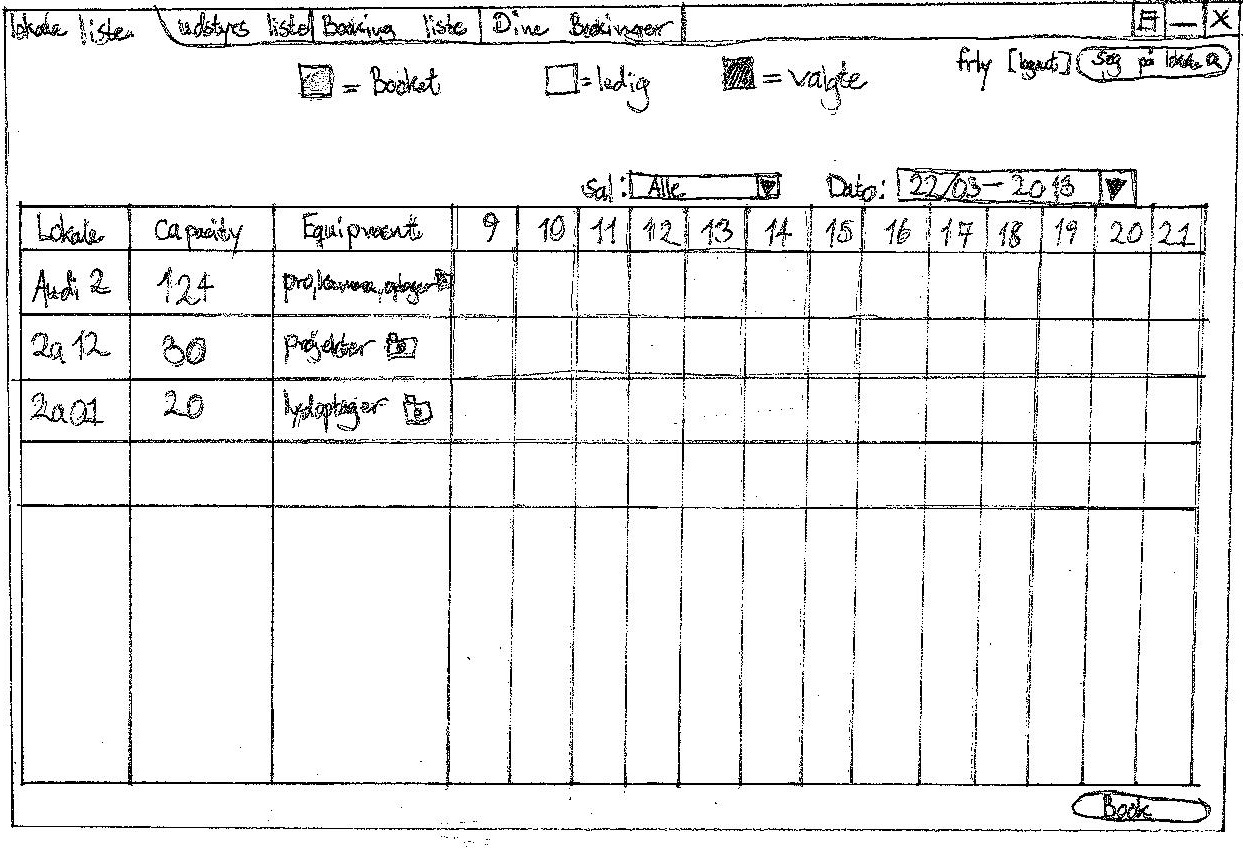
\includegraphics[width=0.5\textwidth, angle=90]{Appendix/GUI-Prototype/PaperMockup/LokaleListe_001}
  \caption{Første udgave af gitter layoutet}
\label{Design_G_Development_FirstGrid}
\end{figure}

\begin{figure}[h!]
  \centering
    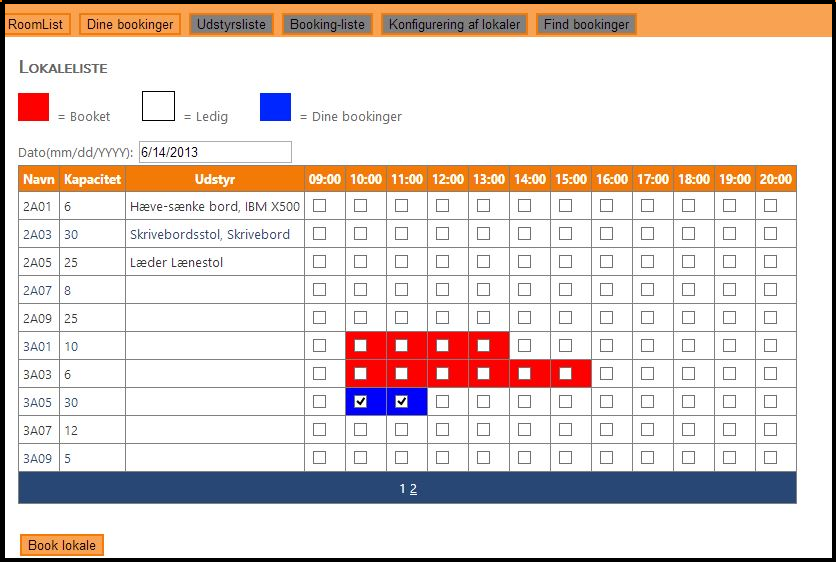
\includegraphics[width=0.5\textwidth]{Appendix/GUI-Prototype/DigitalMockup/GridEksempel}
  \caption{Den endelige udgave af gitteret}
\label{Design_G_Development_FinalGrid}
\end{figure}

Hvis man markere et lokale i det tidsrum man gerne vil booke det og trykker book vil bookingen blive oprettet og man vil blive navigeret videre til en side der visser en oversigt over alle dine bookinger, se figur\ref{Design_G_Development_YourBookings_Final}. 

Til designet af det skærmbillede fokuserede vi på at overholde Gestalt-lovene\cite[s. 68]{SL_UID}, specifikt Law of Proximity\footnote{"Pieces that are close together are perceived as belonging together".}, da vi gerne ville opnå, at det virkede intuitivt for brugeren, at det var de knapper der skulle bruges til at interegere med gitteret. 

\begin{figure}[h!]
  \centering
    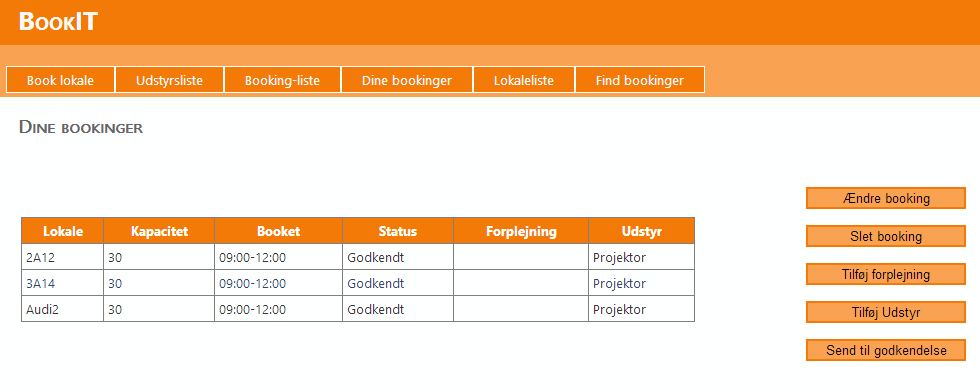
\includegraphics[width=0.5\textwidth]{Appendix/GUI-Prototype/DigitalMockup/DineBookinger}
  \caption{Skærmbilledet til visning af bookinger}
\label{Design_G_Development_YourBookings_Final}
\end{figure} 

Figur\ref{Design_G_Development_Forplejning_Final} viser det endelige skærmbilled til forplejnings valg. Til designet af skærmbillede fokuserede vi på, at det grafisk skulle minde om \ref{Design_G_Development_FinalGrid således, at vi overholdte designregel 1 på den måde ville brugeren intuitivt vide hvordan man skulle tilføje forplejning. De samme design beslutninger gælder for tilføjelse af udstyr til en booking, skærmbilledet kan ses i  \ref{Appendix} på side \pageref{Appendix}.

\begin{comment}
\begin{figure}[h!]
  \centering
    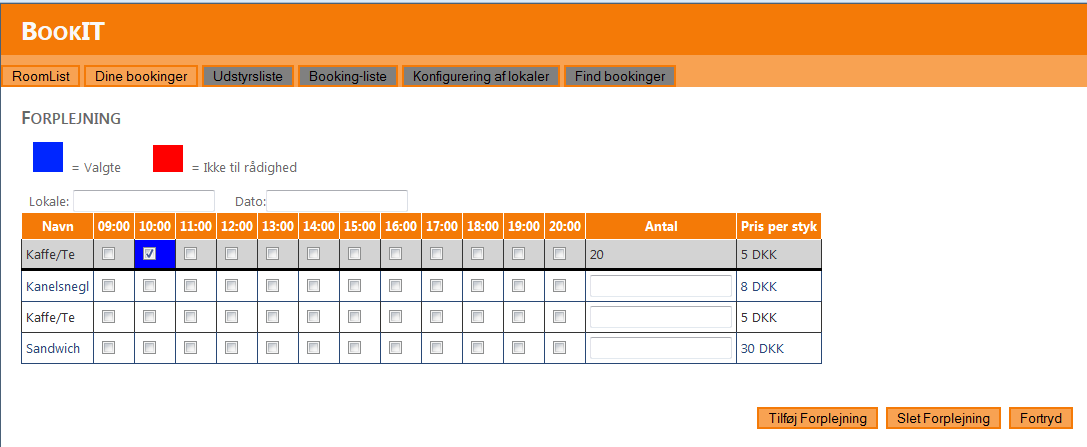
\includegraphics[width=0.5\textwidth]{Appendix/GUI-Prototype/DigitalMockup/Forplejning}
  \caption{Skærmbilledet til booking af forplejning}
\label{Design_G_Development_Forplejning_Final}
\end{figure} 
\end{comment}
\subsection{Bookingliste}
For at en bruger kan tilføje udstyr eller forplejning til sin booking skal den først godkendes. Dette gøres af recepsionisten, som har en liste over alle bookinger som brugerne har oprettet, se figur \ref{Design_G_Development_BookingListe_Final}. Til det endelig design af skærmbilledet valgt vi at flytte godkend/afvis knapperne fra inde i gitteret, som de var i papermockupen se figur \ref{Design_G_Development_BookingListe}, til at være ved siden af gitteret således at vi ligesom i figur\ref{Design_G_Development_YourBookings_Final} benyttede "Law of proximity". Desuden havde ingen af de andre gittre knapper i sig, så vi vurderede, at det så vidt muligt skulle være ens på alle billeder således, at vi overholdt designregel 1.

\begin{comment}
\begin{figure}[h!]
  \centering
    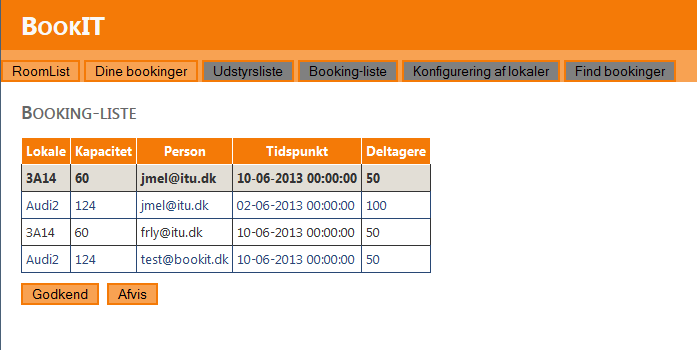
\includegraphics[width=0.5\textwidth]{Appendix/GUI-Prototype/DigitalMockup/BookingListe}
  \caption{Skærmbilledet af recepsionistens liste af bruger bookinger.}
\label{Design_G_Development_BookingListe_Final}
\end{figure} 
\end{comment}

\begin{figure}[h!]
  \centering
    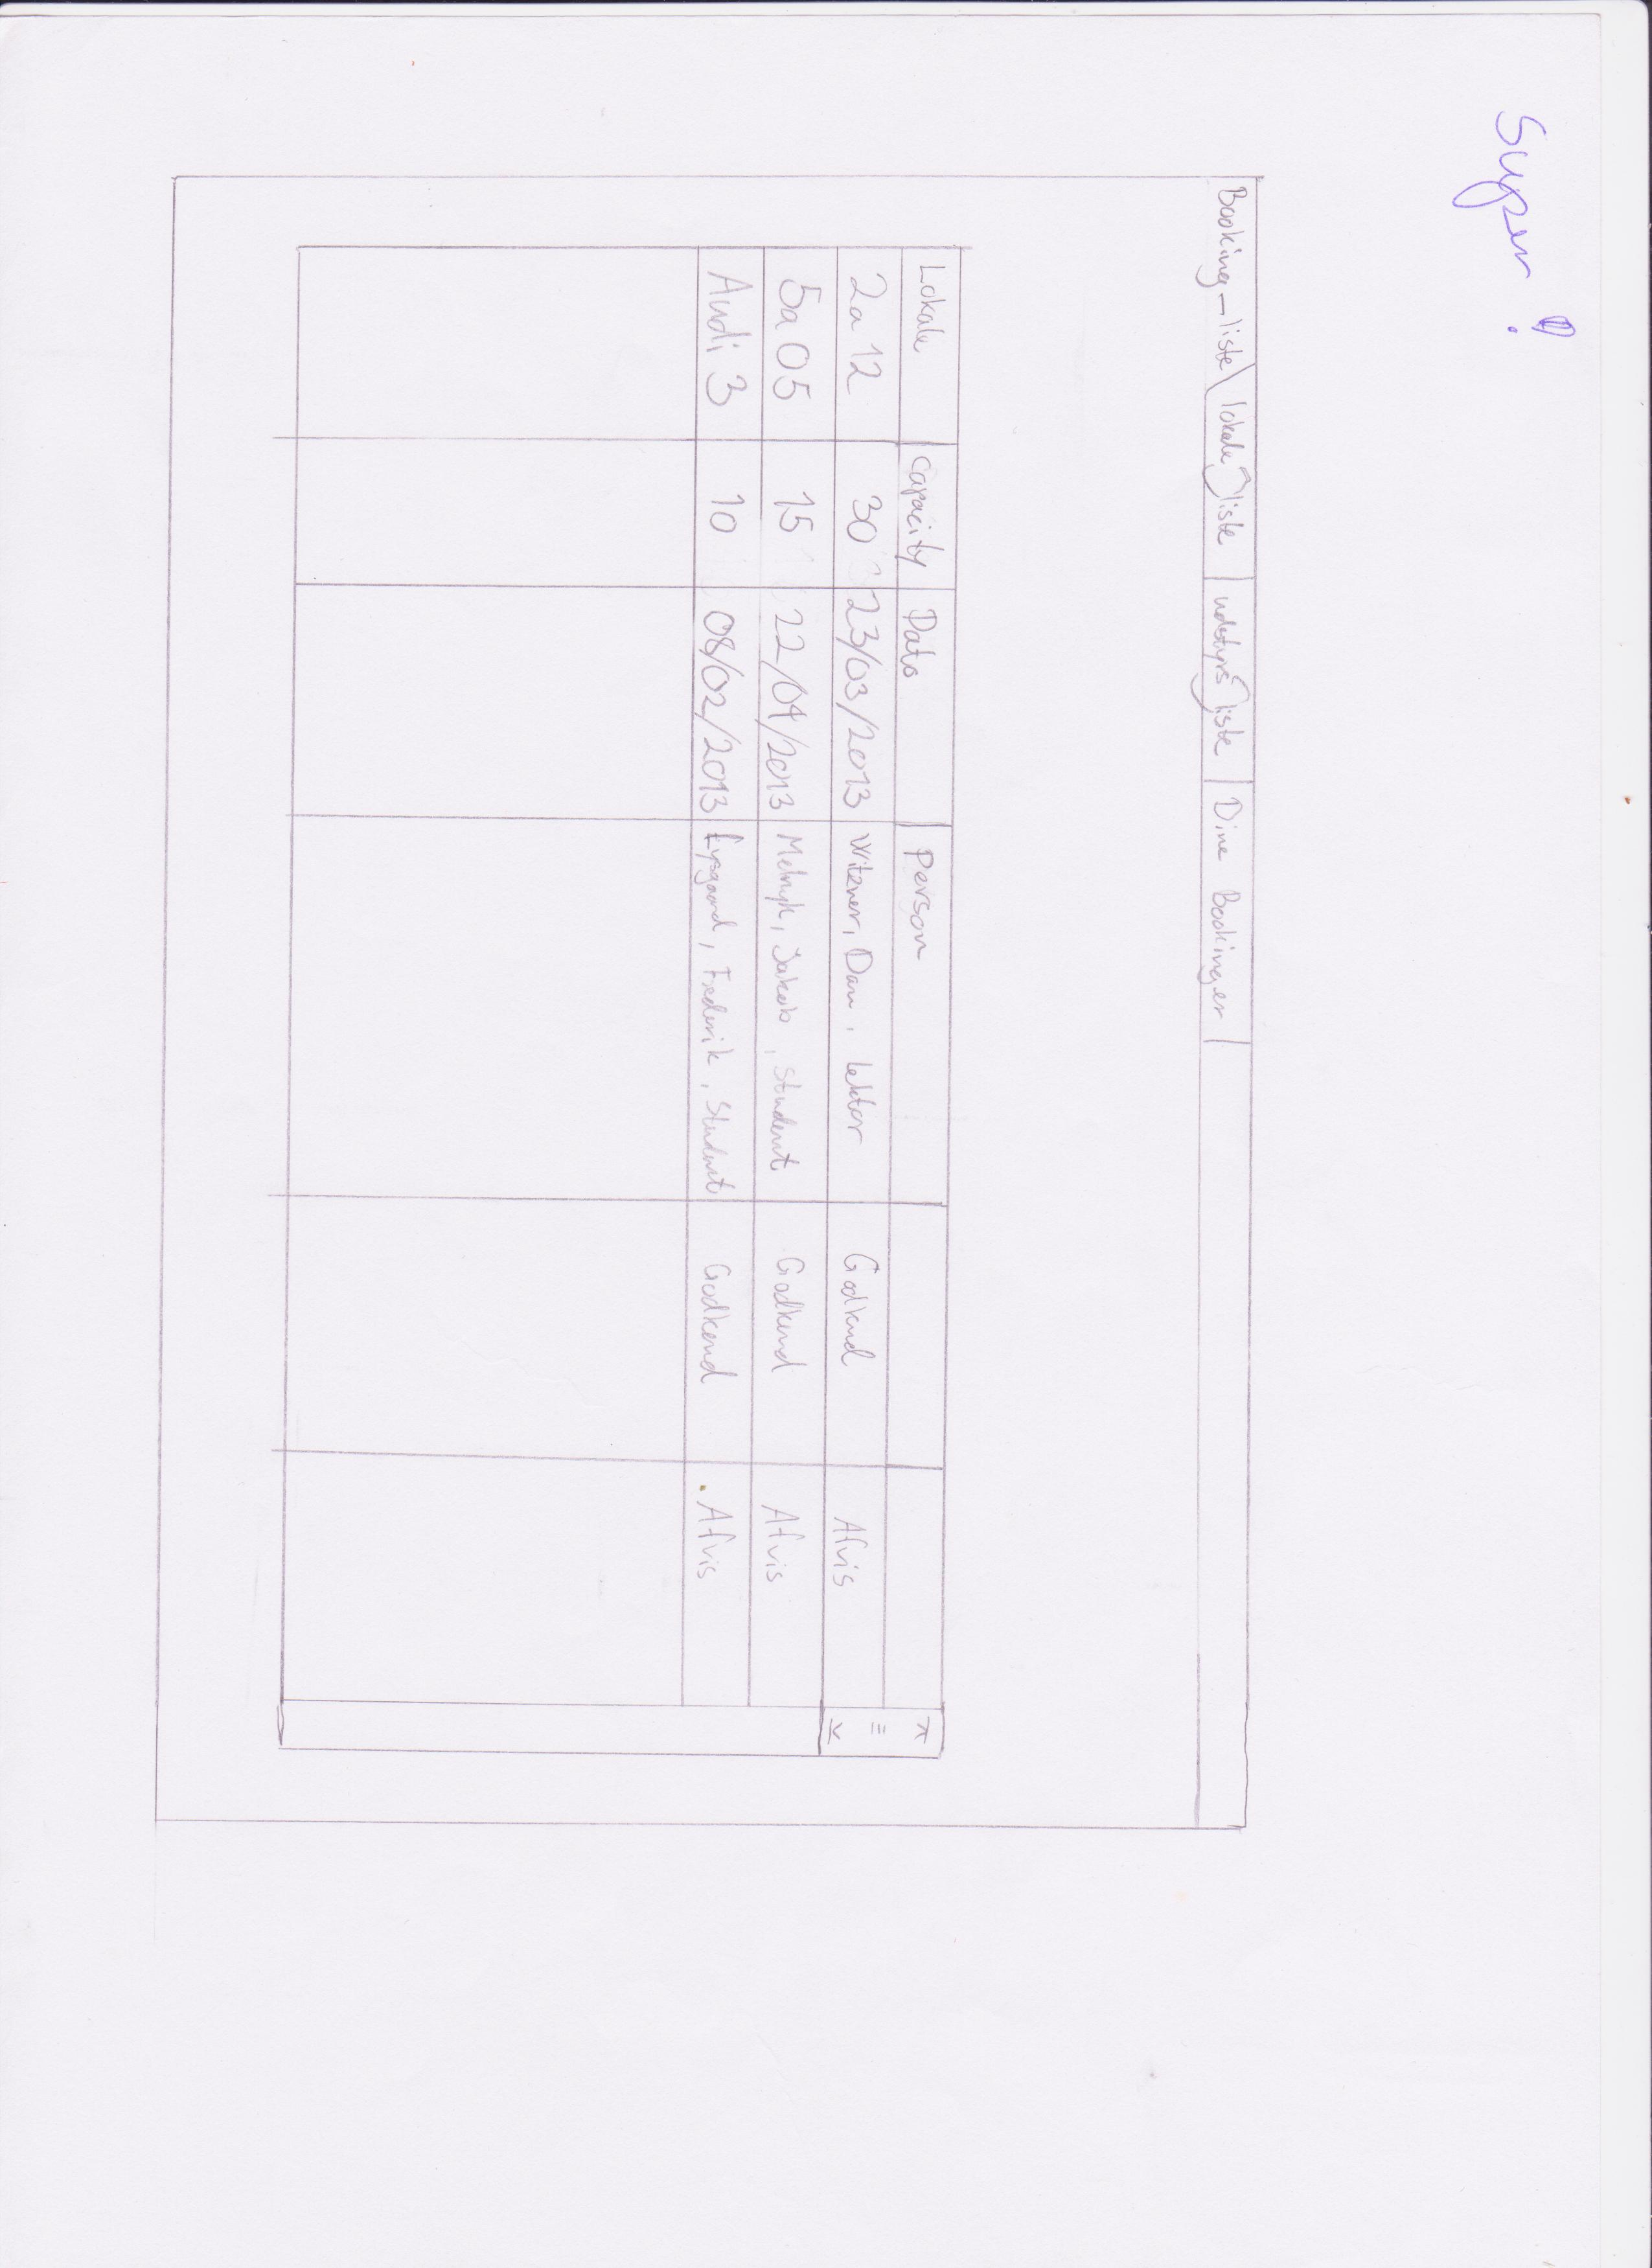
\includegraphics[width=0.5\textwidth]{Appendix/GUI-Prototype/PaperMockup/GodkendBookinger_001}
  \caption{Papermockup af recepsionistens liste af bruger bookinger.}
\label{Design_G_Development_BookingListe}
\end{figure} 

\subsection{Udstyrsliste}
Figuren \ref{Design_G_Development_BookingListe_Final} viser det endelige skærmbillede af listen over udstyr og tilføjelse af nyt udstyr til systemet. Til designet af skærmbilledet brugte vi "Law of proximity" så det er tydeligt, at de to funktionaliteter i skærmbilledet ikke hører sammen. Den eneste ændring der er blevet lavet til det endelige skærmbillede  i forhold til den originale papermockup\ref{Appendix} på side \pageref{Appendix} er, at der er blevet tilføjet en checkbox, hvor man kan vælge om udstyret skal kunne udlånes. Hvis den ikke udfyldes vil udstyret blive kvalificeret som inventar og det vil derfor ikke blive vist under muligt udstyr, der kan tilføjes en booking. 

\begin{comment}
\begin{figure}[h!]
  \centering
    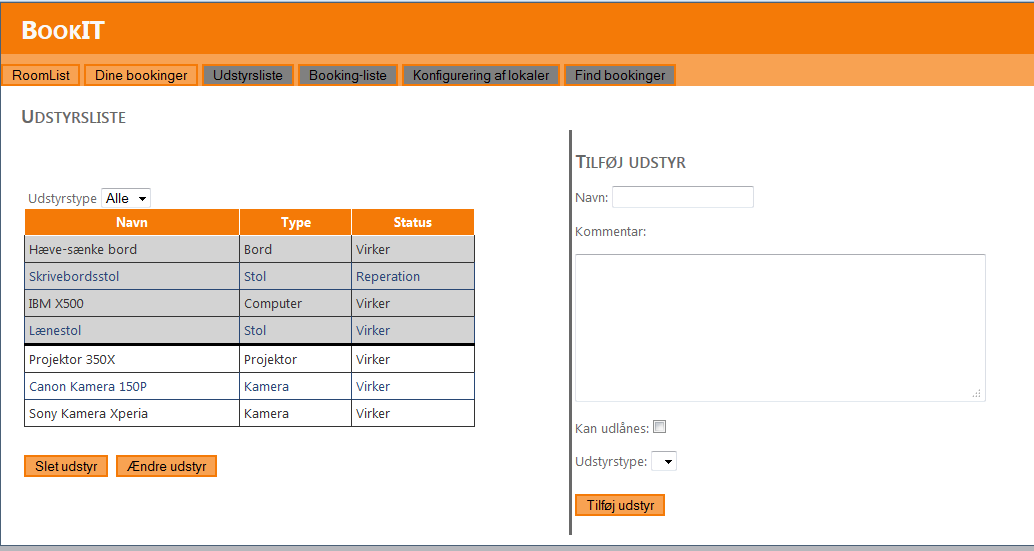
\includegraphics[width=0.5\textwidth]{Appendix/GUI-Prototype/DigitalMockup/UdstyrsListe}
  \caption{Skærmbilledet af recepsionistens liste over udstyr i ITUs system.}
\label{Design_G_Development_UdstyrsListe_Final}
\end{figure} 
\end{comment}

\subsection{Lokale liste}
I systemet er der også mulighed for ændre i listen over lokaler, se figur \ref{Design_G_Development_LokaleListe_Final}. Til designet af skærmbilledet fokuserede vi på, at der skulle være klart overblik, vi sørgede derfor for at overholde law of proximity ved at ligge knapperne tæt på gitteret, hvilket også gør, at det kun er det vigtige information der bliver præsenteret i gitteret.

\begin{comment}
\begin{figure}[h!]
  \centering
    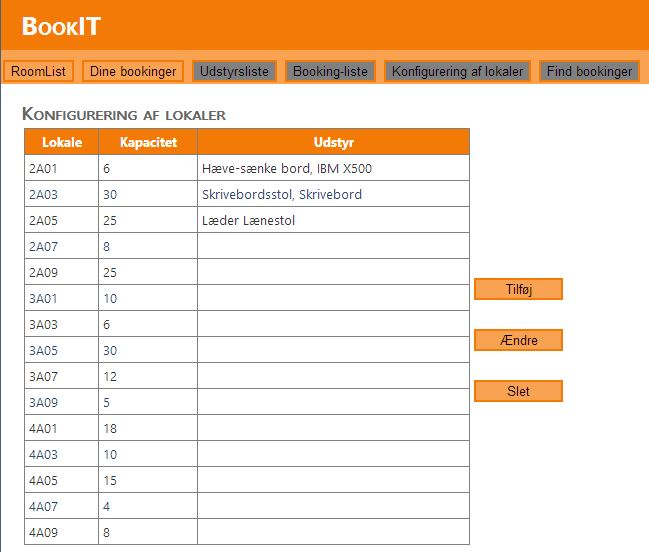
\includegraphics[width=0.5\textwidth]{Appendix/GUI-Prototype/DigitalMockup/LokaleListe}
  \caption{Skærmbilledet af recepsionistens liste over lokaler i ITUs system.}
\label{Design_G_Development_LokaleListe_Final}
\end{figure} 
\end{comment}

\subsection{Ændring af lokale}
Til ændring af lokaler i systemet fokuserede vi på, at man skulle være i stand til at ændre de basale ting som navn og kapacitet, og samtidig være i stand til, at se en liste over inventar i lokalet hvor man skulle kunne tilføje eller fjerne udstyr. Til papermockupen, se figur \ref{Design_G_Development_AendreLokale} havde vi skærmbilledet opdelt i tre afsnit, et til at skifte kapcitet og navn, et til at tilføje inventar og et til at slette inventar.

Dette var en meget uoverskuelige løsning og den var ikke strømlignet i forhold til resten af GUI'en. Vi valgte at lave en løsningen som var i stil med de andre skærmbilleder se figur \ref{Design_G_Development_AendreLokale_Final} vi valgte, at skærmbilledet kun skulle være fokuseret på en gitterløsning hvor den øverste del ville være det udstyr der allerede var i lokalet og resten af gitteret ville så være fyldt med udstyr som man kunne vælge at tilføje til lokalet.

\begin{comment}
\begin{figure}[h!]
  \centering
    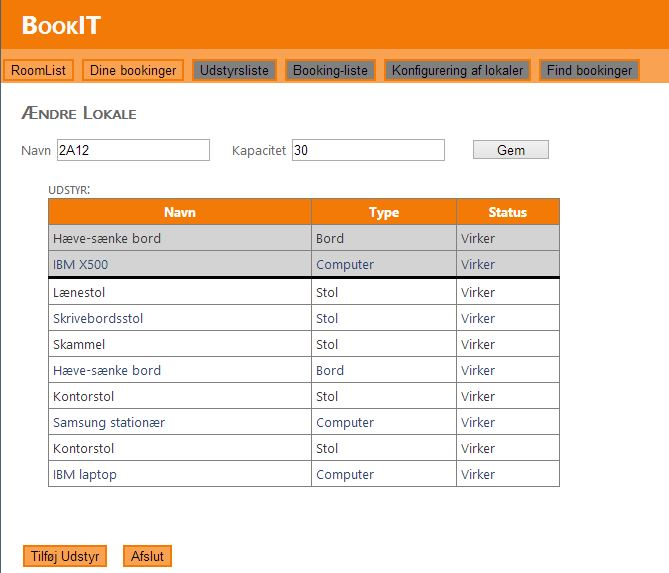
\includegraphics[width=0.5\textwidth]{Appendix/GUI-Prototype/DigitalMockup/AendreLokale}
  \caption{Skærmbilledet til ændring af lokale.}
\label{Design_G_Development_AendreLokale_Final}
\end{figure} 
\end{comment}

\begin{figure}[h!]
  \centering
    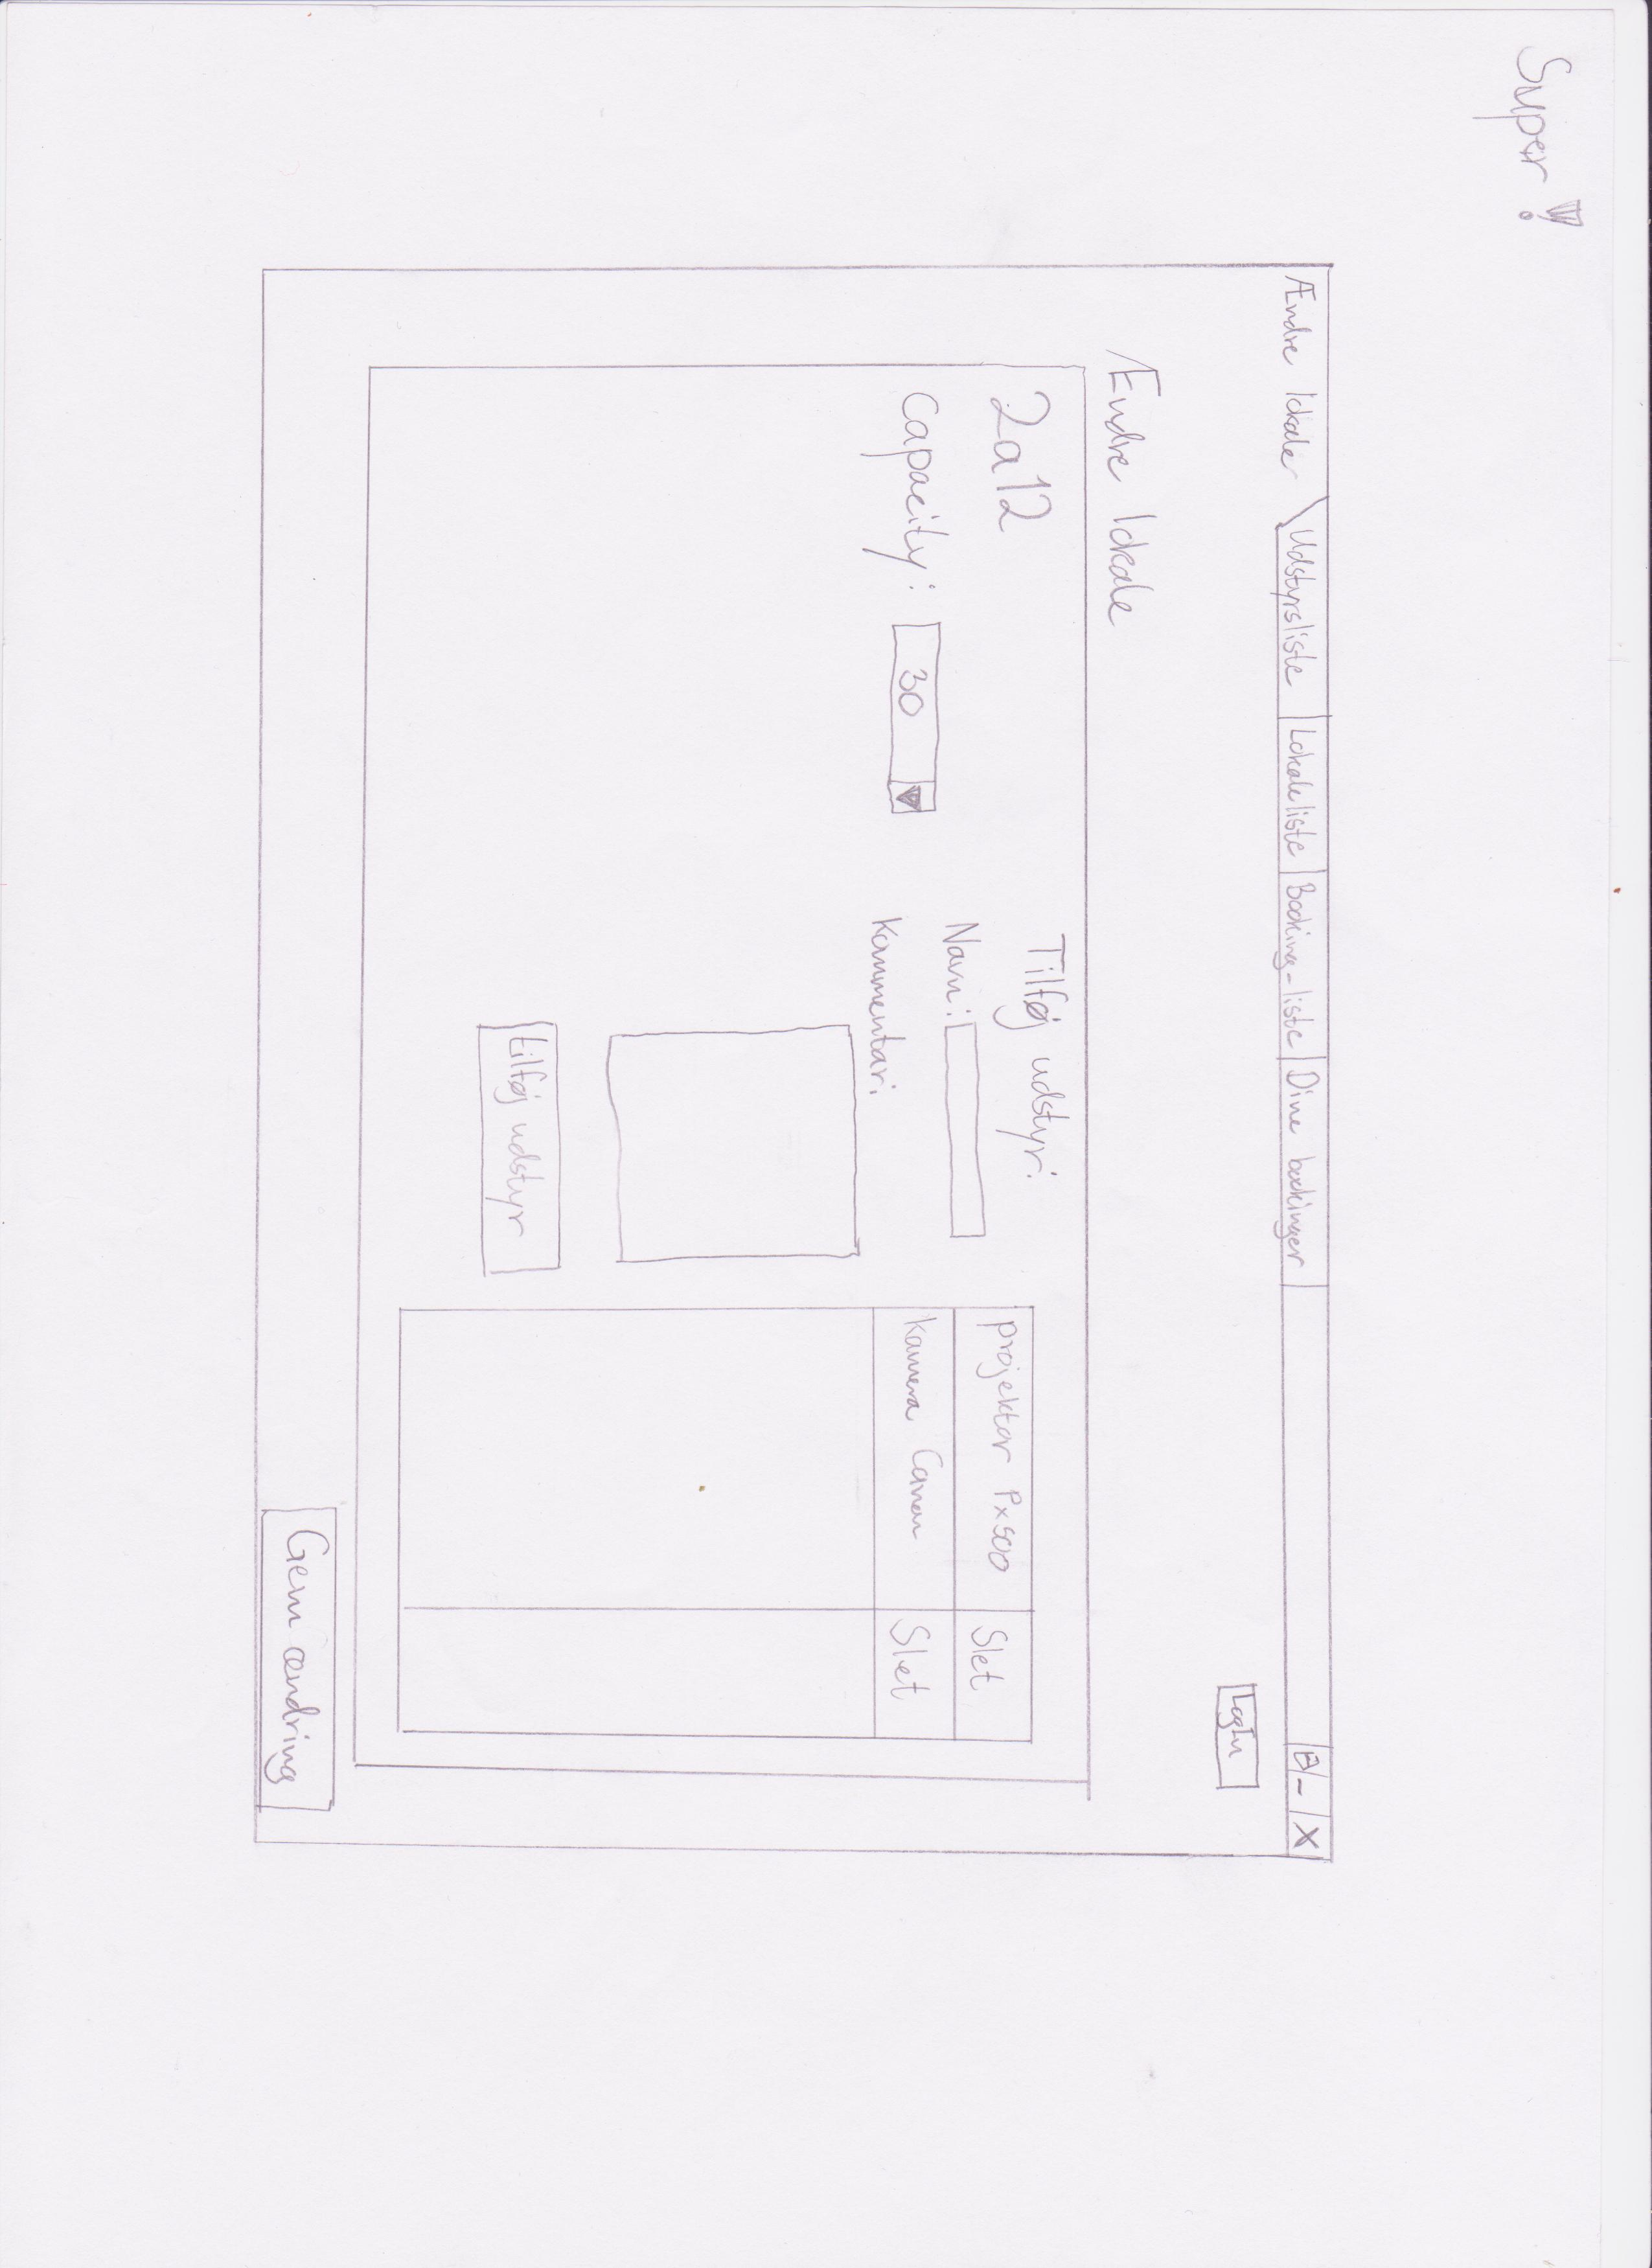
\includegraphics[width=0.5\textwidth]{Appendix/GUI-Prototype/PaperMockup/AendreLokale_001}
  \caption{Papermockup til ændring af lokale.}
\label{Design_G_Development_AendreLokale}
\end{figure} 